\entry{Antecedentes Teóricos}


\section{Formalismo Hamiltoniano para ondas en medios continuos.}
\subsection*{Las bases.}
En el caso más simple posible podemos describir un medio continuo a partir de un par de variables canónicas $q(\vec r, t)$ y $p(\vec r, t)$ de forma tal que las ecuaciones de movimiento serán:

\begin{equation}
	\frac{\partial q}{\partial t} = \frac{\delta \mathcal{H}}{\delta p} \qquad \frac{\partial p}{\partial t} = -\frac{\delta \mathcal{H}}{\delta q}
	\label{eq:Hamilton_continuum}
\end{equation}

Aquí tenemos la densidad Hamiltoniana $\mathcal{H}$, y los $\delta$ representan la \textit{derivada funcional}, análoga a la derivada parcial en el límite continuo. Vamos a tener las propiedades análogas a la versión para variables finitas:

\begin{equation}
	\frac{\delta q(\vec r)}{\delta q(\pvec r')} = \delta^3(\vec r - \pvec r') \qquad \frac{\delta p(\vec r)}{\delta p(\pvec r')} = \delta^3(\vec r - \pvec r')
\end{equation}

Además, aplica la regla de la cadena:

\begin{equation}
	\frac{\delta f(\vec r)}{\delta q(\pvec r')} = \frac{\partial f(\vec r)}{\partial q(\vec r)} \frac{\delta q(\vec r)}{\delta q(\pvec r')} \qquad \frac{\delta f(\vec r)}{\delta p(\pvec r')} = \frac{\partial f(\vec r)}{\partial p(\vec r)} \frac{\delta p(\vec r)}{\delta p(\pvec r')}
\end{equation}

Y conmuta con derivadas parciales de las variables espaciales (e.g. $\partial_{r^i}$) y con integración en variales especiales (e.g. $\int d^3r$).


Además será importante definir el \textbf{corchete de Poisson}. Para un conjunto de variables discretas $(q_i,p_i)$ es (el orden de los dos términos es convención):

\begin{equation}
	\{A, B\} = \sum_i\left(\frac{\partial A}{\partial p_i}\frac{\partial B}{\partial q_i} - \frac{\partial A}{\partial q_i}\frac{\partial B}{\partial p_i}\right)
\end{equation}

De forma que en variables canónicas tenemos:

\begin{equation}
	\{q_i,q_j\}=\{p_i,p_j\}=0 \qquad \{q_i,p_j\} = \delta_{ij}
\end{equation}

Y en el límite continuo esto resulta en:

\begin{equation}
	\{A, B\} = \int d^3r \left(\frac{\delta A}{\delta p}\frac{\delta B}{\delta q} - \frac{\delta A}{\delta q}\frac{\delta B}{\delta p}\right)
\end{equation}

Y la condición de canonicidad queda expresada como:

\begin{equation}
	\{q(\vec r),q(\pvec r')\}=\{p(\vec r),p(\pvec r)\}=0 \qquad \{q(\vec r),p(\pvec r')\} = \delta^3(\vec r- \pvec r')
\end{equation}

Esto es fundamental, ya que las transformaciones canónicas, que preservan la forma de las ecuaciones \eqref{eq:Hamilton_continuum}, serán aquellas que preservan estos corchetes de Poisson ($\{A(q',p'), B(q',p')\}_{q,p}$).


\subsection*{Teoremas de Conservación y simetrías.}
La derivada temporal de una función (con una posible dependencia explícita en $t$) será:

\begin{equation}
	\frac{df(q,p,t)}{dt} = \{H, f\} + \frac{\partial f}{\partial t}
\end{equation}

En general no hay dependencias explícitas, con lo cual tenemos que si $\{H, f\}=0$ entonces la cantidad $f$ es constante de movimiento.



\subsection*{Pasar a variables complejas.}
Ahora bien, se puede mostrar que la siguiente transformación es canónica (a menos de un factor multiplicativo):

\begin{equation}
	a(\vec r,t)=\frac{1}{\sqrt{2}}\big(Q(\vec r,t)+iP(\vec r,t)\big) \qquad a^*(\vec r,t)=\frac{1}{\sqrt{2}}\big(Q(\vec r,t)-iP(\vec r,t)\big)
\end{equation}

Con $Q=\lambda q$ y $P=p / \lambda$ tales que $Q$ y $P$ tengan las mismas unidades. La ventaja de pasar a las variables complejas es que se reduce de las dos ecuaciones \eqref{eq:Hamilton_continuum} a una sola (la segunda es la conjugada de la primera):

\begin{equation}
	i\frac{\partial a}{\partial t} = \frac{\delta \mathcal{H}}{\delta a^*}
\end{equation}

Con los corchetes en las coordenadas originales\footnote{A veces, parece que en las nuevas variables ($\{\cdot,\cdot\}_{a,a^*}$) se escribe el corchete con un factor $i$ adelante}:

\begin{equation}
	\{a(\vec r), a(\pvec r')\}_{Q,P} = \{a^*(\vec r), a^*(\pvec r')\}_{Q,P} = 0 \qquad \{a(\vec r), a^*(\pvec r')\}_{Q,P} = i\delta(\vec r - \pvec r')
\end{equation}

Estas variables complejas son análogas a los operadores de subida y bajada en cuántica. 

\subsection*{Las cantidades conservadas}
En un primer lugar tendremos la conservación de la energía total (siempre que trabajemos con el modelo más sencillo), pero en el caso que el Hamiltoniano tenga simetría $U(1)$ en las variables $a$, habrá otra ley de conservación asociada, $N=|a|^2$, que es análogo al número de partículas en el caso cuántico. Ya desarrollaremos esto más adelante. 

\subsection*{Paso al espacio de Fourier.}
Vamos a imaginar que estamos en una caja de largo $L$ con condiciones de contorno periódicas, que eventualmente podemos hacer tender a infinito, y vamos a expresar a la variable $a(\vec r)$ como una combinación de las variables $a_{\vec k} \equiv a(\vec k)$ tal que:

\begin{equation}
	a_{\vec k} = a(\vec k) = \frac{1}{V}\int d\vec r\;a(\vec r)e^{-i\vec k\cdot\vec r} \qquad a(\vec r) = \sum_{\vec k} a_{\vec k} e^{i\vec k\cdot\vec r}
\end{equation}

Es posible mostrar usando los corchetes para la variable $a$ en el espacio real que las nuevas variables en el espacio de momento $a_{\vec k}$ satisfacen los mismos corchetes de Poisson, a menos de un factor de volumen. Entonces las ecuaciones de movimiento mantienen su forma:

\begin{equation}
	i\frac{\partial a_{\vec k}}{\partial t} = \frac{\delta \mathcal{H}}{\delta a_{\vec k}^*}
\end{equation}

\section{Desarrollo perturbativo del Hamiltoniano.}
Nos va a interesar escribir el Hamiltoniano como una serie de potencias de $a$ y $a^*$. El término de orden 0, i.e. $\mathcal{H}_0$, no es relevante, ya que es una constante que no aparece en la ecuación de movimiento al derivar, y el término de orden 1, $\mathcal{H}_1$, podemos eliminarlo asumiendo que el medio está en equilibrio cuando las amplitudes de las ondas son 0, y el mínimo está en $a=a^*=0$. De esta forma nos queda:

\begin{equation}
	\mathcal{H} = \mathcal{H}_2 + \mathcal{H}_3 + \mathcal{H}_4 + \cdots \equiv \mathcal{H}_2 + \mathcal{H}_{int}
\end{equation}

Donde $\mathcal{H}_{int}$ representa las interacciones entre ondas. 
\subsection*{El orden más bajo.}

Se puede mostrar que existe una transformación canónica a unas nuevas variables $b_{\vec{k}},b_{\vec{k}^*}$ tales que \cite{zakharovKolmogorovSpectraTurbulence1992}:

\begin{equation}
	\mathcal{H}_2 = \int \omega(\vec k)b_{\vec k}b^*_{\vec k}
\end{equation} 

De forma tal que a primer orden no nulo la ecuación de movimiento resulta trivial:

\begin{equation}
	\frac{\partial b_{\vec{k}}}{\partial t}=-i\omega b_{\vec{k}} \qquad \Rightarrow{} \qquad b_{\vec{k}}=b(\vec k, 0)e^{-i\omega t}
\end{equation}

En este punto la única diferencia entre distintos medios radica en la relación de dispersión $\omega(\vec k)$.

\subsection*{El Hamiltoniano de interacción.}
Los términos de orden superior se pueden interpretar como términos de interacción entre ondas, en analogía a lo que ocurre en mecánica cuántica. Vamos a usar la notación reducida: $b_{\vec k_1} \equiv b_1$.

Para las interacciones de tres ondas tenemos:

\begin{align}
	\mathcal{H}_3 &= \frac{1}{2}\int\big(V_{123}b^*_1b_2b_3+\text{c.c.}\big)\delta(\vec k_1-\vec k_2 -\vec k_3) d\vec k_1d\vec k_2d\vec k_3 \\ &+ \frac{1}{6} \int\big(U_{123}b^*_1b^*_2b^*_3+\text{c.c.}\big)\delta(\vec k_1 + \vec k_2 + \vec k_3) d\vec k_1d\vec k_2d\vec k_3
\end{align} 

Donde tenemos unos coeficientes $V_{123}$ y $U_{123}$ que nos hablan de la magnitud de la interacción. El primer término describe procesos de la forma $1\rightarrow2$ y  $2\rightarrow1$, mientras que el segundo describe procesos del tipo $3\rightarrow0$ y $0\rightarrow3$, que son aniquilaciones de tres ondas hacia el vacío o creación espontánea de tres ondas por fluctuaciones. % 

Por otro lado, para las interacciones de cuatro ondas tenemos:

\begin{align}
	\mathcal{H}_4 &= \frac{1}{4} \int W_{1234}b1^*b_2^*b_3b_4\delta(\vec k_1+\vec k_2-\vec k_3-\vec k_4) d\vec k_1d\vec k_2d\vec k_3d\vec k_4 \\
	&+\int \big(G_{1234}b_1b_2^*b_3^*b_4^* + \text{c.c.}\big) \delta(\vec k_1-\vec k_2-\vec k_3-\vec k_4) d\vec k_1d\vec k_2d\vec k_3d\vec k_4 \\
	&+\int \big(R^*_{1234}b_1b_2b_3b_4 + \text{c.c.}\big) \delta(\vec k_1+\vec k_2+\vec k_3+\vec k_4) d\vec k_1d\vec k_2d\vec k_3d\vec k_4
\end{align}

Donde ahora tenemos procesos del tipo $2\rightarrow2$ para el primer término, $1\rightarrow3$ y $3\rightarrow1$ para el segundo, $4\rightarrow0$ y $0\rightarrow4$ para el tercero.
 
Los coeficientes de interacción van a tener las simetrías asociadas a la interacción, o sea, se van a poder intercambiar los índices asociados a "partículas" de cada lado de la flecha, por ejemplo, $V_{123}=V_{132}$.

Notemos además que si hay presentes términos con una cantidad distinta de "partículas" de un lado que del otro entonces no habrá simetría $U(1)$ y no se conservará la cantidad de partículas asociadas a ese proceso. 


\subsection*{Interacciones Resonantes de $N$ ondas} % 
En general vamos a poder tener interacciones de tanta cantidad de ondas como querramos, a medida que aumentemos el orden del Hamiltoniano de interacción. Éstas son integrales de colisiones como las de la Ecuación de Boltzmann.

Ahora bien, en general va a ser suficiente con llegar al primer término no nulo, tal que se satisfagan la conservación de lo que en cuántica serían el momento y la energía: 

\begin{equation}
	\vec k_1 \pm \vec k_2 \pm \cdots \pm \vec k_N = 0 \qquad \omega(\vec k_1) \pm \omega(\vec k_2) \pm \cdots \pm \omega(\vec k_N) = 0
	\label{eq:condición_resonancia}
\end{equation}

Los signos corresponderán a si la "partícula" ingresa o sale. 

Si no se satisface la segunda condición de resonancia entonces el término correspondiente del Hamiltoniano puede eliminarse mediante transformaciones canónicas apropiadas, como se verá más adelante \cite{zakharovKolmogorovSpectraTurbulence1992}.

Para el caso en que tenemos una relación de dispersión del tipo $\omega\sim k^{\alpha}$ la condición de resonancia de tres ondas no será posible en los casos en que $\alpha<1$, con lo cual el primer término resonante será el de cuatro ondas, para el cual siempre hay solución en el caso de $\omega\sim k^{\alpha}$. La demostración se puede entender gráficamente, si dibujamos las superficies en 2D para $\omega(\vec k, \vec k_0)$ y $\omega(\vec k) + \omega(\vec k_0)$, donde $\vec k_0$ es un parámetro que puede variarse. Si las curvas se intersecan hay solución, sino solo existe la solución trivial en que ambas curvas son iguales, para el caso en que una de las ondas es 0. Esto está ilustrado en la Figura \ref{fig:solución_condición_resonante}. % STO 

\begin{figure}[!ht]
	\begin{minipage}[c]{0.5\textwidth}
		\begin{subfigure}{\textwidth}
			\centering
			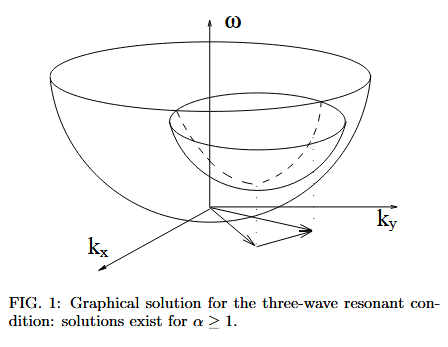
\includegraphics[width=0.678\textwidth]{Figures/Antecedentes_teoricos/Resonancia_alpha_mayor}
			\captionsetup{width=0.8\textwidth}
			\subcaption{}
		\end{subfigure}
	\end{minipage}\begin{minipage}[c]{0.49\textwidth}
		\begin{subfigure}{\textwidth}
			\centering
			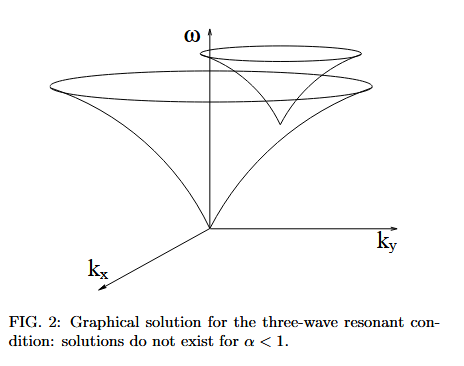
\includegraphics[width=0.76878\textwidth]{Figures/Antecedentes_teoricos/Resonancia_alpha_menor1}
			\captionsetup{width=0.8\textwidth}
			\subcaption{}
		\end{subfigure}
	\end{minipage}
	\caption{Soluciones gráficas para la condición resonante para dos casos distintos de la relación de dispersión $\omega\sim k^{\alpha}$.}
	\label{fig:solución_condición_resonante}
\end{figure}

Para las ondas de gravedad $\alpha=1/2$ con lo cual las interacciones resonantes de 3 ondas no están permitidas (sino serían ondas con energía negativa).

\section{Eliminación de los términos no resonantes.}
Vamos a querer mostrar que efectivamente en el caso de que un término sea no resonante, o sea, que no cumple la condición \eqref{eq:condición_resonancia}, existirá una transformación canónica a nuevas variables $c_{\vec k}, c_{\vec k}^*$ en las cuales ese término no aparece en el Hamiltoniano de interacción. 

A modo ilustrativo \cite{zakharovKolmogorovSpectraTurbulence1992} plantea para una sola variable el Hamiltoniano hasta orden cuatro:

\begin{equation}
	\mathcal{H} = \omega bb^*+\frac{V}{2}(b^2b^*+{b^*}^2) + \frac{U}{6}(b^3+{b^*}^3) + \frac{W}{4}(b^2{b^*}^2) + G(b^3b^*+b{b^*}^3) + R (b^4+{b^*}^4)
\end{equation}

Y pide que la nueva variable sea de la forma (desarrollo perturbativo en $b$):

\begin{equation}
	b = c + A_1c^2+A_2cc^*+A_3{c^*}^2 + B_1c^3+B_2c^*c^2+B_3c{c^*}^2+B_4{c^*}^3+\cdots
\end{equation}

Luego pide que $\{b,b^*\}_{c,c^*}=1$ para que la transformación sea efectivamente canónica y resuelve para los coeficientes $A_i$ y $B_i$ pidiendo que todos los términos no lineales del Hamiltoniano excepto $c^2{c^*}^2$ sean 0. Entonces llega a que:

\begin{equation}
	\mathcal{H} = \omega cc^* + \frac{1}{4} Tc^2{c^*}^2 \qquad T=W-\frac{3V^2}{\omega}-\frac{U^2}{3\omega}
\end{equation}

O sea, que siempre y cuando $\omega \neq 0$ se pueden eliminar los términos no resonantes del Hamiltoniano. 

Es posible hacer exactamente lo mismo para el caso en que no hay triadas resonantes, quedando: 

\begin{equation}
	\mathcal{H} = \frac{1}{4} \int T_{1234} c_1^*c_2^*c_3c_4\delta(\vec k_1+\vec k_2 - \vec k_3 - \vec k_4) d\vec k_1d\vec k_2 d\vec k_3 d\vec k_4
\end{equation}

Donde el coeficiente de interacción resulta:

\begin{align}
	T_{1234} = W_{1234} &-\frac{U_{-1-212}U_{-3-434}}{\omega_3+\omega_4+\omega_{3+4}} + \frac{V^*_{1+212}V_{3+434}}{\omega_1+\omega_2-\omega_{1+2}} 	-\frac{V^*_{131-3}V_{424-2}}{\omega_{4-2}+\omega_2-\omega_4} \\ 
	&- \frac{V^*_{242-4}V_{313-1}}{\omega_{3-1}+\omega_1-\omega_3} 
	-\frac{V^*_{232-3}V_{414-1}}{\omega_{4-1}+\omega_1-\omega_4}-\frac{V^*_{141-4}V_{323-2}}{\omega_{3-2}+\omega_2-\omega_3} 
\end{align} 

Notemos que si efectivamente la condición resonante para tres ondas no puede cumplirse (con una relación de dispersión de no decaimiento), entonces los denominadores de $T_{1234}$ no divergen y efectivamente se puede eliminar $\mathcal{H}_3$ del Hamiltoniano de interacción $\mathcal{H}_{int}$.

En general la prohibición de interacciones del tipo $2\rightarrow1$ y $1\rightarrow2$ implican la prohibición de los términos $1\rightarrow3$ y $3\rightarrow1$. Igualmente se eliminan los términos $4\rightarrow0$ y $0\rightarrow4$ del Hamiltoniano, resultando en su versión más simplificada.


Notemos que al interactuar la mitad de las ondas de cada lado ($N/2\rightarrow N/2$) se conserva la cantidad de partículas, asociado a la simetría $U(1)$ que mencionamos antes:

\begin{equation}
	N = \int c^*_{\vec k}c_{\vec k} d\vec k
	\label{eq:Wave_action_integral}
\end{equation}

Que es lo que se conoce como la integral de \textit{Wave action}.


Los distintos términos de $T_{1234}$ se pueden interpretar gráficamente:

\begin{figure}[!ht]
	\centering
	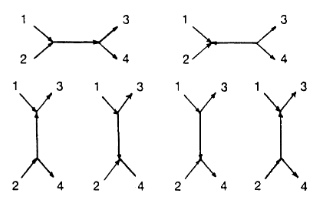
\includegraphics[width=0.7\linewidth]{Figures/Antecedentes_teoricos/Procesos_de_4_ondas}
	\caption{Distintos procesos de cuatro ondas como segundo orden perturbativo a proceso de tres ondas, donde la tercera es virtual y conecta ambos extremos. } % ec
	\label{fig:procesosde4ondas}
\end{figure}


Donde se pueden pensar como un segundo orden de perturbación a un proceso de tres ondas, donde aparece una fuerza virtual que no conserva energía y momento. 

\section{Paso a la estadística y la Ecuación Cinética.}
La idea ahora va a ser pasar de la descripción dinámica del sistema a una estadística en función de las funciones de correlación de las amplitudes de ondas.

\subsection*{Resumen Ecuaciones de Movimiento}
En las variables apropiadas los Hamiltonianos sin términos no resonantes nos quedan, para el caso de tres ondas: 


\begin{equation}
	\mathcal{H}_3 = \frac{1}{2}\int \big(V_{123}c_1^*c_2c_3 + \text{c.c.}\big)\delta(\vec k_1-\vec k_2-\vec k_3)d\vec k_1 d\vec k_2 d\vec k_3
\end{equation}

Con su ecuación de movimiento:

\begin{equation}
	i\frac{\partial c_{\vec k}}{\partial t} - \omega_k c_{\vec k} = \int \left(\frac{1}{2}V_{k12}c_1c_2\delta(\vec k - \vec k_1 -\vec k_2) + V^*_{1k2}c_1c_2^*\delta(\vec k_1 -\vec k-\vec k_2)\right)d\vec k_1d\vec k_2
\end{equation}

Donde primero tenemos $k\rightarrow1+2$ (que es una sola opción) y luego $k+2\rightarrow1$ (que son dos opciones).

Y para el caso de cuatro ondas:

\begin{equation}
	\mathcal{H} = \frac{1}{4}\int T_{1234}c_1^*c_2^*c_3c_4\delta(\vec k_1+\vec k_2-\vec k_3-\vec k_4)d\vec k_1 d\vec k_22 d\vec k_3 d\vec k_4
\end{equation}

Con su ecuación de movimiento:

\begin{equation}
	i\frac{\partial c_{\vec k}}{\partial t} - \omega_k c_{\vec k} = \frac{1}{2} \int T_{k123}c_1^*c_2c_3\delta(\vec k+\vec k_1-\vec k_2-\vec k_2) d\vec k_1 d\vec k_2d\vec k_3
\end{equation}

Que son procesos $2\rightarrow2$.

\subsection*{Paso a la estadística.}
Las ecuaciones de movimiento anteriores son para la evolución temporal de las amplitudes y fases de $c_{\vec k} = |c(\vec k, t)|e^{i\phi(\vec k, t)}$. En el caso en que las nolinealidades son débiles y hay una gran cantidad de modos esta evolución suele ser redundante, ya que incluye la dinámica rápida de $\phi\sim\omega t$ que deja a la evolución lenta de las amplitudes (que es constante en el caso puramente lineal, orden más bajo) virtualmente no afectada. Por esto vamos a querer pasar a una descripción estadística, donde solo trabajaremos con las funciones de correlación para $c_{\vec k}$, donde vamos a promediar en un ensamble.

Vamos a asumir una "caotización" de las fases, de forma tal que aunque al inicio estuvieran correlacionadas, luego de un tiempo ya no lo estarán. Podemos pensar que esto se debe a la dispersión del medio o a que inicialmente están en un equilibrio muy inestable del cual los saca cualquier perturbación del medio. De esta forma, bajo la aproximación de fases aleatorias tenemos las correlaciones:

\begin{align}
	\langle c_{\vec k}\rangle &= \langle |c_{\vec k}|e^{i\phi_{\vec k}}	 \rangle = 0 \\
	\langle c_{\vec k} c_{\pvec k'} \rangle &= \langle |c_{\vec k}||c_{\pvec k'} e^{i(\phi_{\vec k}+\phi_{\pvec k'})}| = 0 \\
	\langle c_{\vec k} c^*_{\pvec k'} \rangle  &= \langle |c_{\vec k}||c_{\pvec k'} e^{i(\phi_{\vec k}-\phi_{\pvec k'})}| = n(\vec k) \delta(\vec k - \pvec k')
\end{align} 

Acá definimos la acción de onda $n(\vec k) = c_{\vec k}c^*_{\vec k}$, que sería la densidad de "partículas" con número de onda $\vec k$ en la integral \eqref{eq:Wave_action_integral}.  

Por último para los correlatorres de una cantidad impar siempre van a dar 0, y para los de orden 4 y 6 tenemos:

\begin{align}
	\langle	c_1^*c_2^*c_3c_4 \rangle & = n_1 n_2 \big[\delta_{1-3}\delta_{2-4} + \delta_{1-4}\delta_{2-3}\big] \\ 
	\langle c_1^*c_2^*c_3^*c_4c_5c_6 \rangle &= n_1n_2n_3\big[  \delta_{1-4}\delta_{2-5}\delta_{3-6} + \delta_{1-4}\delta_{2-6}\delta_{3-5} + \delta_{1-5}\delta_{2-4}\delta_{3-6} \\ 
	& +\delta_{1-5}\delta_{2-6}\delta_{3-4} + \delta_{1-6}\delta_{2-4}\delta_{3-5} + \delta_{1-6}\delta_{2-5}\delta_{3-6} \big] 
\end{align}

Que básicamente las deltas dan que queden dos o tres  $n$'s.

\subsection*{Ecuación cinética de tres ondas.}



\subsection*{Ecuación cinética de cuatro ondas.}




\section{Correspondencia con fluidos con superficie libre.}



\section{Espectro de energía y PSD.}
Nos interesará estudiar la transferencia de energía entre escalas experimentalmente, que estará caracterizada por la densidad espectral de energía $E_k$ tal que la magnitud $E = \int E_k dk$ se conserva. 

Para esto vamos a empezar dando las definiciones básicas de lo que estaremos usando.

Como mencioné anteriormente, la energía total va a venir dada por una distribución, que puede escribirse ya sea en el espacio de $k$ o de $\omega$, vinculados ambos a través de la relación de dispersión lineal $\omega(k)$. Entonces:

\begin{equation}
	E = \int E(\vec k) d\vec k = \int k E(\vec k) dkd\theta \equiv \int E(k) dk = \int E(\omega) d\omega
\end{equation}

O sea, estamos definiendo $E(k) = 2\pi E(\vec k)$ y la relación entre las densidades en espacio de frecuencia y momento está dada por: $E(k) dk = E(\omega) d\omega$.

Esta energía será la de la superficie libre. En principio sabemos que se dará un balance entre la energía cinética y la potencial, como una especie de equipartición \cite{kunduFluidMechanics2014}. Se suele calcular la potencial (a partir de las mediciones para la superficie libre $\eta$) y se multiplica por 2 \cite{deikeEtudesExperimentalesNumeriques2013}. Vamos a entonces trabajar con las energías potenciales, cuya expresión depende de si tenemos ondas de gravedad o capilares. Tenemos que:

\begin{equation}
	E_p^g = \frac{1}{2} \rho g \int \eta^2 dS \qquad E_p^s = \gamma \int\sqrt{1+(\nabla\eta)^2} - 1 dS
\end{equation}

Acá la energía por capilaridad es básicamente la integral del elemento de superficie $ds$. Se puede aproximar a primer orden para una onda armónica en el caso lineal (con $eta\ll1$), entonces \cite{deikeEtudesExperimentalesNumeriques2013}

\begin{equation}
	E_p^s = \frac{1}{2} \gamma\int k^2\eta^2dS
\end{equation}

Usando que $(1+\varepsilon)^n\approx1+n\varepsilon$. Ahora vamos a querer pasar al espacio de Fourier, transformando las energías:

\begin{equation}
	E_p^g = \frac{\rho g}{2} \int |\eta_{\vec k}|^2d\vec k \qquad E_p^s = \frac{\gamma}{2} \int k^2|\eta_{\vec k}|^2d\vec k
\end{equation}

Donde $\eta_{\vec k}$ es la transformada de Fourier de $\eta$:

\begin{equation}
	\eta(\vec k) = \frac{1}{2\pi}\int\eta(\vec r)e^{-i\vec k\cdot\vec r} d\vec r
\end{equation}

Podemos integrar en cilíndricas para definir $\eta_k = 2\pi k\eta_{\vec k}$. Las densidades espectrales de energía van a ser los integrandos. 

Por último vamos a definir la Power Spectral Density (PSD) que va a ser lo más sencillo para trabajar experimentalmente:

\begin{equation}
	S_\eta(\omega) = \frac{1}{T} |\eta_\omega|^2 \qquad S_\eta(k) = \frac{1}{L^2} |\eta_k|^2
\end{equation}

Acá ahora $\eta(\omega) = \frac{1}{\sqrt{2\pi}}\int\eta(t)e^{i\omega t}$ es la transformada de Fourier respecto al tiempo. Además para obtener ya sea $\eta(t)$ o $\eta(\vec r)$ se puede promediar en el tiempo o espacio, con lo cual en realidad sería $S_\eta\propto\langle |\eta|^2 \rangle$ (y técnicamente el promedio sería en el ensamble, pero consideramos al sistema ergódico). \cite{falconExperimentsSurfaceGravity2022}

Podemos relacionar las PSD en ambos espacios como $S(\omega)d\omega=S(k)dk$. De esta forma entonces podemos obtener la densidad de energía a partir de la PSD como:

\begin{equation}
		E^g(k) = \frac{\rho g}{2} S_\eta(k) \qquad E^s(k)=\frac{\gamma}{2}k^2S_\eta(k)
\end{equation}


Una cosa interesante es que si escribimos explícitamente $S_\eta(k) \propto k|\eta_{\vec k}|^2$ entonces nos queda en ambos casos:

\begin{equation}
	E(k) \propto \omega^2|\eta_{\vec k}|^2 \propto |\dot \eta_{\vec k}|^2 
\end{equation}

Que sería la energía cinética efectivamente.










\section{Espectro de Kolmogorov-Zakharov-Filonenko.}
Experimentalmente es posible observar que el espectro de energía para la elevación de la superficie libre en un determinado rengo de números de ondas (de equilibrio) resulta $E_\omega  \sim A\omega^s$. En este rango la mayor contribución a la dinámica se debe a los efectos no lineales, ya que los viscosos son menores. Es posible calcular los exponentes de forma analítica a partir de las ecuaciones para la superficie libre \cite{zakharovEnergySpectrumStochastic1967}

La densidad de energía se puede escribir como:

\begin{equation}
	E(\vec k) = \omega(\vec k) n(\vec k)
\end{equation}  

Donde $n$ es la \textit{wave action}, análoga a la cantidad de partículas (o ondas) con ese número de onda.

\subsection*{Ondas de gravedad \cite{zakharovEnergySpectrumStochastic1967}}
Tenemos que $E(\omega)=\omega^4n(\omega)$ y pueden calcular que para $n(\omega)=A\omega^s$ hay soluciones $s=-1$, que se corresponde con la distribución de Rayleigh-Jeans (equilibrio termodinámico para el caso lineal, con PDF Gaussiana \cite{nazarenkoWaveTurbulence2011}), y $s=-8$ que es la análoga al espectro de Kolmogorov para turbulencia hidrodinámica.

Las equivalencias son \cite{falconExperimentsSurfaceGravity2022}:

\begin{equation}
	E_k^g \sim P^{1/3} g^{1/2} k^{-5/2} \qquad S_k^g \sim P^{1/3} g^{-1/2} k^{-5/2} \qquad S_\omega^g  \sim P^{1/3} g \omega^{-4}
\end{equation}  

Es posible llegar a estos resultados de forma dimensional, pero para que el exponente sea único hay que asumir a priori que el flujo en el espectro de energía va en el orden $P^{1/(N-1)}$ con $N$ el número de ondas interactuantes más bajo, siendo $N=4$ para ondas de gravedad.

Para hacer los cambios hay que usar la relación de dispersión:

\begin{equation}
	\omega^2=gk
\end{equation}

\subsection*{Ondas de capilaridad \cite{zakharovWeakTurbulenceCapillary1971}}
Al igual que para las ondas de gravedad calculan $n(\omega)$, llegando esta vez a los resultados de $s=-1$ que es la de Rayleigh-Jeans y $s=-17/6$ que es la que nos interesa. Con esto:

\begin{equation}
	E_k^s \sim P^{1/2} \left(\frac{\gamma}{\rho}\right)^{1/4} k^{-7/4} \qquad S_k^s \sim P^{1/2} \left(\frac{\gamma}{\rho}\right)^{-3/4} k^{-15/4} \qquad S_\omega^s  \sim P^{1/2} \left(\frac{\gamma}{\rho}\right)^{1/6} \omega^{-17/6}
\end{equation}   

Acá la relación de dispersión es:

\begin{equation}
	\omega^2 = \frac{\gamma}{\rho}k^3
\end{equation}



\section{Doble cascada para $N$ par} % a sub 
A partir de los resultados para los espectros KZF se puede ver que existe una cascada directa de energía, sin embargo, para el caso en que las interacciones se dan entre un número par de ondas, tenemos otro invariante además de la energía, que es la \textit{wave action}, que tendrá una cascada inversa. \cite{nazarenkoWaveTurbulence2011}

Para el caso de ondas de gravedad, con interacciones de 4 ondas, tenemos el espectro:

\begin{equation}
	E^g_k \sim g^{2/3} \zeta^{1/3} k^{-7/3}
\end{equation}

Con $\zeta$ el flujo de \textit{wave action} (ratio de disipación)

%Estos son los antecedentes Teóricos. Más antecedentes.
%
%Esta es una ecuación:
%
%\begin{equation}
%	A = B + \phi
%	\label{eq:eq_1}
%\end{equation}
%
%Y esta es u referencia a la ecuación \eqref{eq:eq_1}. 
%
%Y por último una prueba del auto-guardado en Github. Y una más. 
%Y esta sería la última. 

% IMÁGENES Y TABLAS
%
% A la izquierda 
% \begin{figure}[!ht]
%	     \begin{minipage}[c]{0.5\textwidth}
%		         \centerfloat
%		         \includegraphics[width=0.8\textwidth]{}
%		     \end{minipage}
%	         \begin{minipage}[c]{0.49\textwidth}
%		         \captionsetup{width=\textwidth}  
%		         \caption{.}
%		     \label{fig:}
%		     \end{minipage}
%	 \end{figure}
%
%A la derecha
% \begin{figure}[!ht]
%	     \begin{minipage}[c]{0.5\textwidth}
%		           \captionsetup{width=\textwidth}  
%		           \caption{.}
%		           \label{fig:}
%		     \end{minipage}
%	     \begin{minipage}[c]{0.49\textwidth}
%		         \centerfloat
%		         \includegraphics[width=0.8\textwidth]{}
%		     \end{minipage}
%	 \end{figure}
% 
% Ancho completo
% \begin{figure}[!ht]
%	     \centerfloat
%	     \includegraphics[width=0.9\textwidth]{}
%	     \caption{}
%	     \label{fig:}
%	 \end{figure}
%
% Wrapfigure
% \begin{wrapfigure}{r}{0.5\textwidth}
%	         \vspace{-20pt}
%	         \centerfloat
%	         \includesvg[width=0.3\textwidth]{}
%	         \captionsetup{width=0.45\textwidth}
%	         \caption{.}
%	         \label{fig:}
%	 \end{wrapfigure}
%
% Generador de tabals: https://www.tablesgenerator.com/
% Tablas con líneas más gruesas: https://tex.stackexchange.com/questions/41758/how-can-i-reproduce-this-table-with-thick-lines
% 
% Tabla y figura (https://tex.stackexchange.com/questions/417505/table-just-below-a-figure)
% \begin{minipage}{0.99\textwidth}
%	   \begin{minipage}[c]{0.49\textwidth}
%		         \centerfloat
%		         \includegraphics[width=\textwidth]{}
%		         \centering
%		         \captionsetup{width=.8\linewidth}
%		         \captionof{figure}{.}
%		         \label{fig:}
%		   \end{minipage}
%	   \hfill
%	   \begin{minipage}[c]{0.49\textwidth}
%		         \centerfloat
%		         \includegraphics[width=\textwidth]{}
%		         \centering
%		         \captionsetup{width=.8\linewidth}
%		         \captionof{table}{.}
%		          \label{tab:}
%		     \end{minipage}
%	 \end{minipage}
% 
% Subfiguras
%\begin{figure}[!ht]
%	\begin{minipage}[c]{0.5\textwidth}
%		\begin{subfigure}{\textwidth}
%			\centering
%			\includegraphics[width=0.8\textwidth]{}
%			\captionsetup{width=0.8\textwidth}
%			\subcaption{.}
%			\label{fig:}
%		\end{subfigure}
%	\end{minipage}\begin{minipage}[c]{0.49\textwidth}
%		\begin{subfigure}{\textwidth}
%			\centering
%			\includegraphics[width=0.8\textwidth]{}
%			\captionsetup{width=0.8\textwidth}
%			\subcaption{.}
%			\label{fig:}
%		\end{subfigure}
%	\end{minipage}
%	\caption{}
%	\label{fig:}
%\end{figure}
% 
% Tablas/figuras iguales side by side
% \begin{table}[]
%	     \parbox{0.5\textwidth}{
%		     \centering
%		     \includegraphics[width=0.95\linewidth]{}
%		     \caption{}
%		     \label{tab:}
%		 }
%	 \parbox{0.5\textwidth}{
%		     \centering
%		     \includegraphics[width=0.9\linewidth]{}
%		     \caption{}
%		     \label{tab:}
%		 }
%	 \end{table}
% 
% Tablas ancho completo
% \begin{table}[!h]
%	     \centerfloat
%	     \caption{.}
%	     \label{tab:}
%	 \end{table}